\chapter{Background Research: Recommender Systems}

This section introduces the fundamental concepts and techniques of recommender systems. Then, it discusses the adoption of recommender systems in research and enterprises. Finally, it gives two examples of algorithms commonly used in recommender systems.

\section{Concepts}

\citet{ricci11} write that traditional recommendations can be observed in various scenarios, such as a peer's recommendation when buying a book or reviews when choosing a movie. The authority of the recommender has an important role in the acceptance of the recommendation. A renowned film critic may appear more credible than a random colleague. When it comes to car parts, a mechanist may be a good candidate to ask. However the authority is not only limited to expertise -- in fact we tend to rely more on recommendations which put our personal experiences and preferences into account. A previous companion for a wonderful trip can certainly have a better authority than a travel agent.

As mentioned in the introduction, with the growth of the Internet, the amount of information available on the Web increased rapidly. Especially, major e-commerce Web sites were extending their range of products and services. Although a wider and varied range of items is initially good for the user, users found it more and more difficult to find the appropriate items or make the right choices. Web sites have deployed different type of solutions -- such as search engines and more user friendly interfaces -- to cope with this problem.

Another approach are recommender systems which basically provides a bespoke collection of items with the intention to highlight relevant items to a user. Depending on the recommending technique used various data sources are taken into account like the user's context or previous interactions. This is a continuous learning process. The more the recommender system learns, the more accurate the recommendations will become. The user's behaviour on given recommendations are further a powerful learning source for the system -- e.g. if the user tends to accept some recommendations over others -- to tweak the recommendations. Most recommender systems concentrate on guiding the user towards novel, unexperienced items \cite{herlocker04}.



\section{Techniques}

In the course of development different techniques to building recommendations emerged. Fundamentally techniques are classified by the information sources they use. The sources of personalised recommendations are typically user-item interactions (\textit{collaborative filtering}), item features (\textit{content-based filtering}), user features (\textit{demographic filtering}) as well as knowledge about the user and item (\textit{knowledge-based filtering}). Non-personalised recommendations also exist in form of ranked lists such as top sellers or related items. However they are typically not part of the research in recommender systems.

\citet{anand03} differentiate between \textit{explicit} and \textit{implicit} data collection. Information the user intentionally provides to the system to express a positive preference to items are referred to as \textit{explicit} data collection including rating an item, adding it to a wish list or liking it. \textit{Implicit} data on the other hand is collected by observing the user's behaviour e.g. usage of navigation and search elements or purchase of items.

\subsection{Collaborative Filtering}
\label{bg-tech-collaborative}

\begin{figure}[ht]
    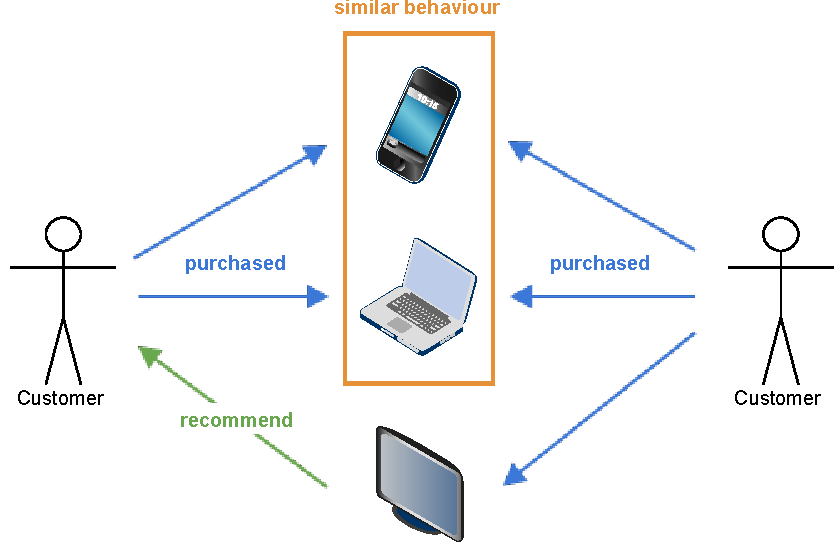
\includegraphics[width=0.7\textwidth,center]{background/techniques/collaborative.pdf}
    \caption{Collaborative Filtering}
    \label{fig:collaborative}
\end{figure}

Basically this technique recommends items other users with similar preferences interacted with e.g. liked or purchased. In order to do this the recommender system needs to observe users' behaviours and interactions. Based on these learnings, it will then look up other users with similar behaviour patterns and build recommendations from their preferences -- preferably items which the active user has not experienced yet (see figure \ref{fig:collaborative}).

The major advantage of the collaborative filtering approach is that the recommender system does not require any knowledge about the items.

Figure \ref{fig:collaborative} illustrates a scenario where the active customer has purchased several items in the past. The recommender system understands that the active customer is similar to another as both have purchased the phone and laptop. Then, the system computes items the similar customer purchased but the active customer has not. It therefore recommends the TV to the first customer.

\subsubsection{Item-to-Item Collaborative Filtering}
\label{bg-tech-itembased}

\begin{figure}[ht]
    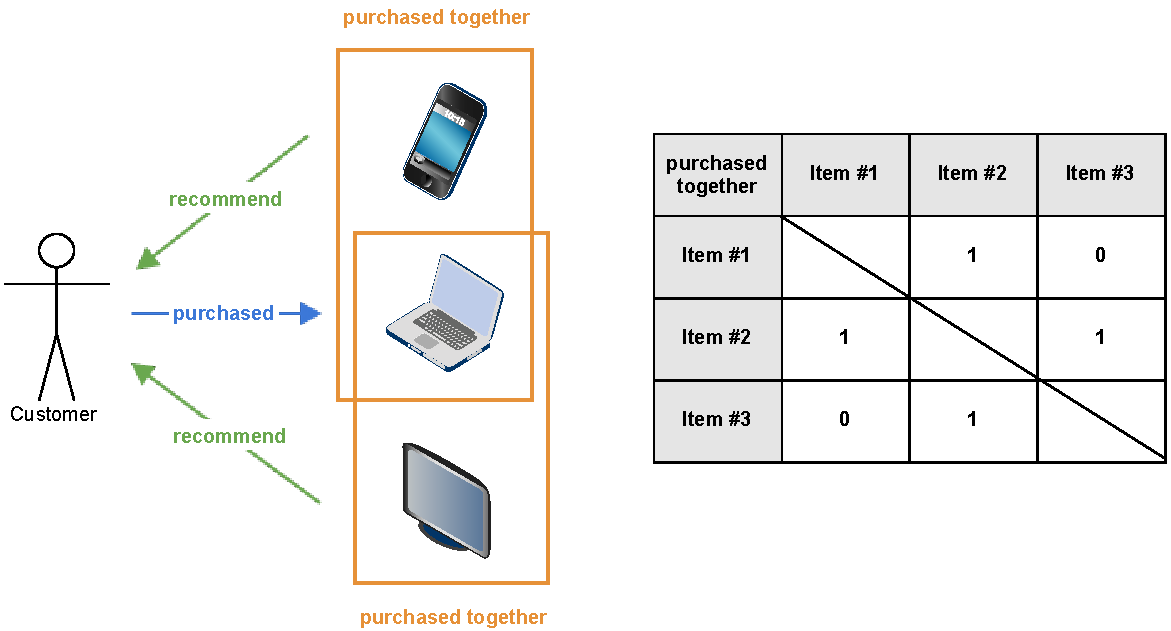
\includegraphics[width=0.7\textwidth,center]{background/techniques/itembased.pdf}
    \caption{Item-to-Item Collaborative Filtering}
    \label{fig:itembased}
\end{figure}

This approach is a derivative of traditional collaborative filtering methods and has been popularised by Amazon \cite{linden03}. The fundamental difference lies in the fact that the item-to-item approach collects collaborative data to put items into relation with other items rather than users. The recommendation query takes an item -- currently viewed or from a wish list -- as an argument and looks for items purchased together with that item (see figure \ref{fig:itembased-amazon}).

Given that the item range can be very wide, item-to-item filtering methods require significant computing time and data storage. However they are usually preprocessed offline thus queries can be processed rather quickly.

Figure \ref{fig:itembased} demonstrates a customer who has purchased an item in the past. The recommender system looks up items which were purchased together with that item and recommends them to the customer.

\subsection{Contentbased Filtering}

\begin{figure}[ht]
    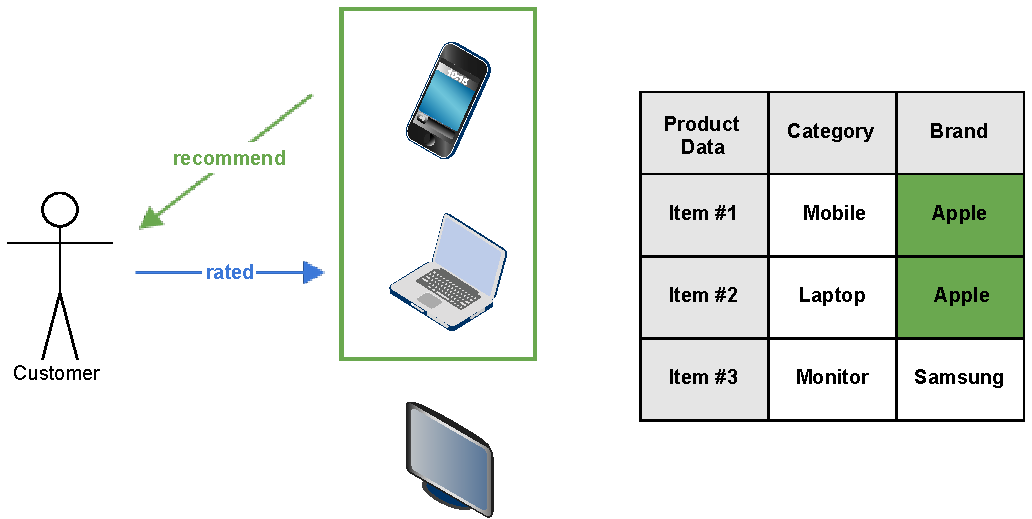
\includegraphics[width=0.7\textwidth,center]{background/techniques/contentbased.pdf}
    \caption{Contentbased Filtering}
    \label{fig:contentbased}
\end{figure}

Content-based recommendation methods make use of item features to find similar items. Based on items the user has showed a positive preference to before -- such as rated or purchased -- other similar items are looked up based on the item's features. Figure \ref{fig:contentbased} illustrates a customer who has rated an item positively. The recommender system compares the rated item with other items, finds another item which has the same brand and therefore recommends that item.

\subsection{Demographic Filtering}

\begin{figure}[ht]
    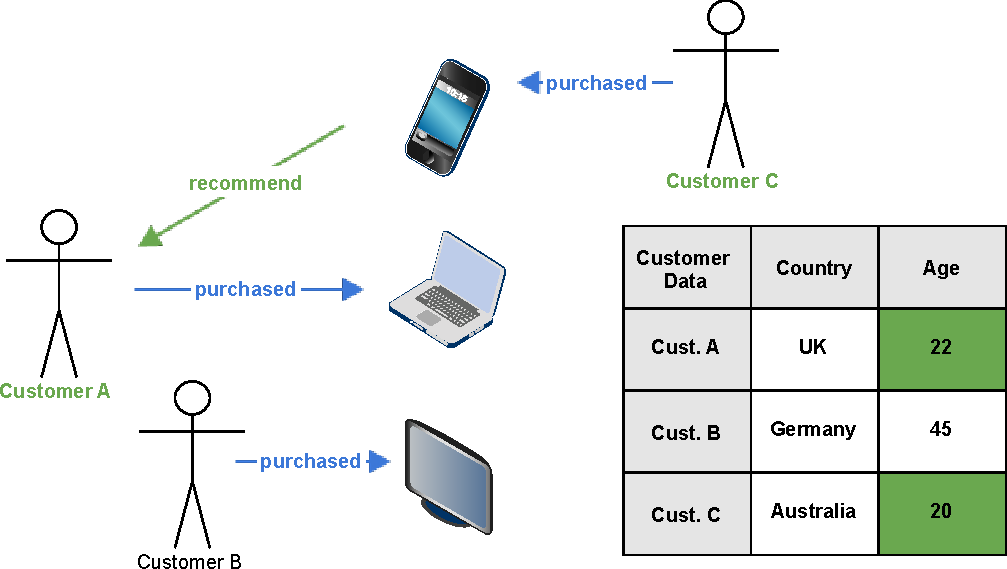
\includegraphics[width=0.7\textwidth,center]{background/techniques/demographic.pdf}
    \caption{Demographic Filtering}
    \label{fig:demographic}
\end{figure}

The demographic filtering is similar to the content-based method with the significant difference that demographic filtering examines the demographic profile of a user -- user features rather than item features -- to find similar users and recommend items those users have showed positive preference to in the past. \citet{burke07} makes the assumption that recommendations should be different for demographic groups. The demographic profile can consist of age, gender, interests, language, country etc. To give an example, a hotel search engine may want to recommend different hotels to a business person and different ones for a young couple.

Figure \ref{fig:demographic} shows how a demographic filtering recommender system would recommend an item to customer A based on a customer base of three customers with previous purchase history. The recommender analyses the customer profile features and eventually decides relying on the age feature that customer C is similar to customer A. Hence the system recommends a product customer C purchased in the past.

\subsection{Knowledgebased Filtering}

\begin{figure}[ht]
    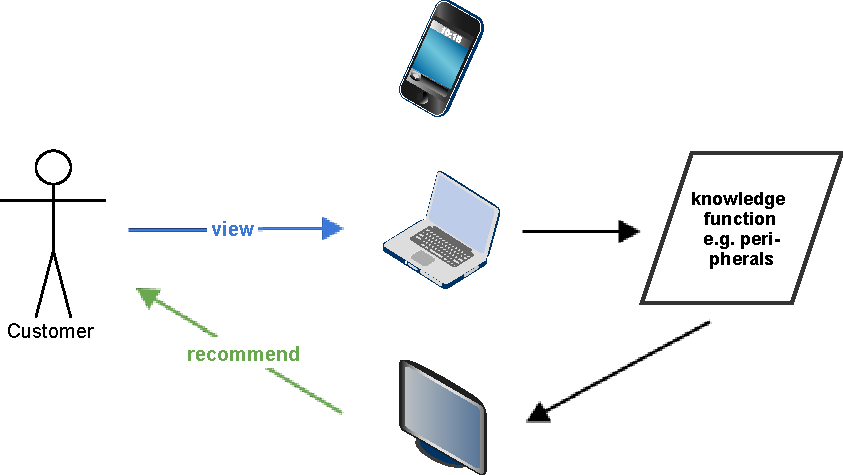
\includegraphics[width=0.7\textwidth,center]{background/techniques/knowledgebased.pdf}
    \caption{Knowledgebased Filtering}
    \label{fig:knowledgebased}
\end{figure}

Recommendations of knowledge-based systems rely on specific domain knowledge to determine useful items for a user. These systems are usually constraint-based or case-based. Both approaches are similar in their conversational process. In other words, the user specifies the requirements and the system tries to find solutions which are fulfilling them. Whereas constraint-based systems are matching the requirements explicitly (such as price ranges), case-based systems make use of similarity measures (e.g. distance to a point of interest) \cite{ricci11}.

An example of a knowledge-based recommender is figure \ref{fig:knowledgebased} which recommends a monitor as a peripheral to a customer who views a laptop. This is based on explicit knowledge that amongst others external screens are a demand for laptop users.

\subsection{Hybrids}
\label{bg-tech-hybrid}

Hybrid recommender systems make us of two or more individual recommender systems -- hereinafter referred to as components -- to combine aforementioned techniques. One possible motivation of using hybrid systems may be to overcome weaknesses of one approach by combining it with another. However it is also possible to combine systems implementing the same technique but e.g. using different knowledge sources. There are many possible ways of combining techniques of which \citet{burke07} identified seven:

\begin{description}
    \item[Weighted] The scores of recommender components are combined using a linear formula. A score is a numerical rank attached to items.
    \item[Switching] The system chooses one component over another which is based on some criterion.
    \item[Mixed] Recommendations from components are summed up and presented together. Implementations usually differ on how the results are merged together.
    \item[Feature Combination] A contributing component modifies the features of a knowledge source and feeds into the actual recommender component.
    \item[Feature Augmentation] Similar to \textit{feature combination} this approach's contributing component adds new features rather than modify them (see figure \ref{fig:featureaugmenting}).

    \begin{figure}[ht]
        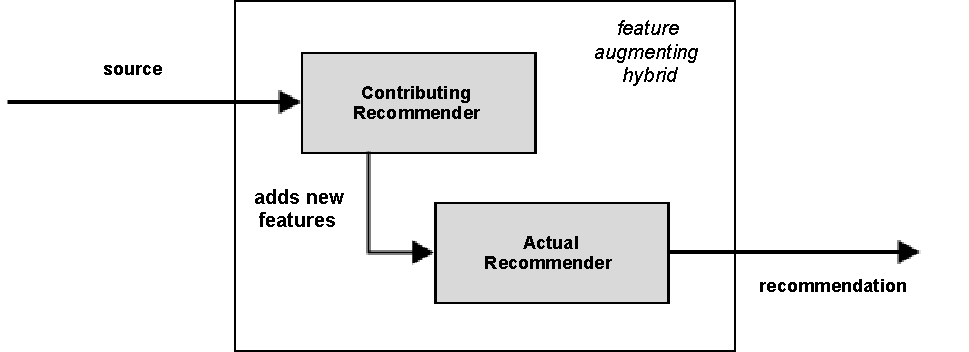
\includegraphics[width=0.7\textwidth,center]{background/techniques/featureaugmenting.pdf}
        \caption{Feature Augmenting Hybrid Recommender System}
        \label{fig:featureaugmenting}
    \end{figure}

    \item[Cascade] Components are given strict priorities with the lower prioritised ones breaking ties of the higher ones.
    \item[Meta-Level] Similar to \textit{feature combination} as well as \textit{feature agumentation}, yet the contributing component completely replaces -- instead of appends or modifies -- the initial source.
\end{description}

\section{Adoption}
\label{bg-adoption}

\citet{ricci11} note that research on recommender systems is relatively new compared to other classical information retrieval methods like databases and search engines. However it is gaining attention due to various reasons. First of all e-commerce companies including Amazon, YouTube and Netflix invest a lot in recommender systems. As trendsetters and pioneers for other institutions they build a demand for further research and development. Dedicated conferences and academic courses as well as its adaption in several academic journals are indicators of recognition of this research area.

E-commerce companies running recommender systems hope among others to increase number of items sold, sell more diverse items, increase customer satisfaction and recommend sequences plus bundles \cite{herlocker04}.

\begin{figure}[ht]
    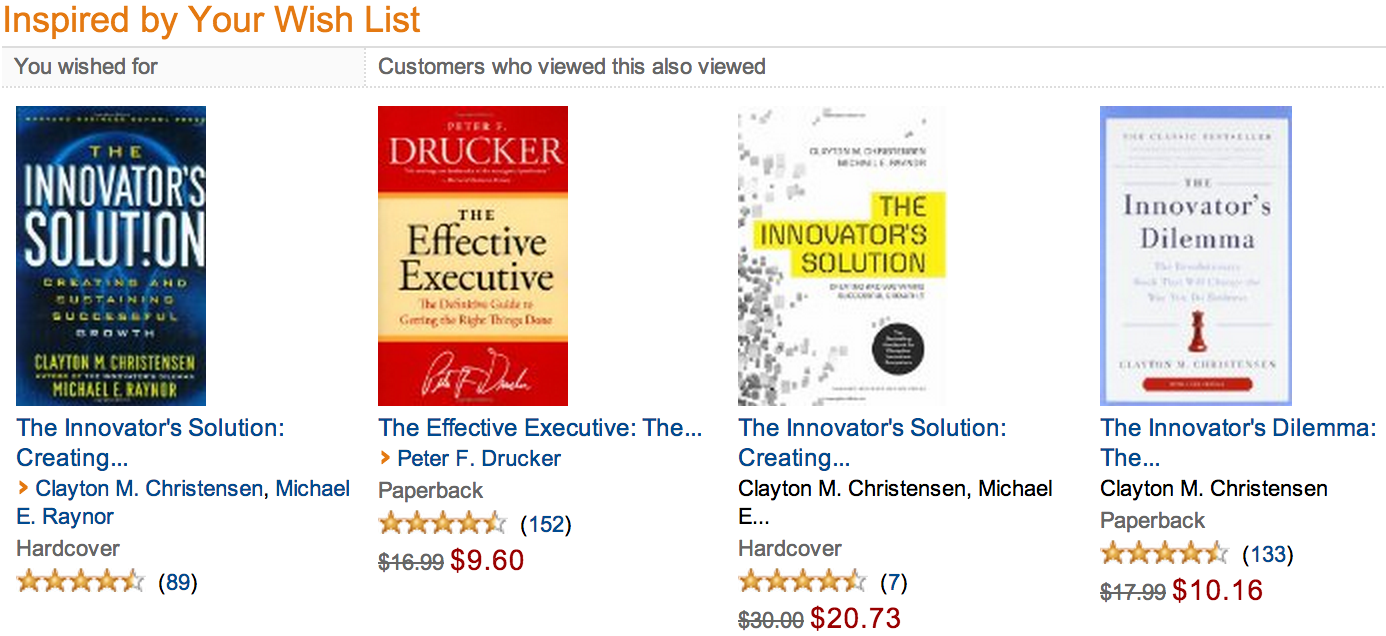
\includegraphics[width=\textwidth,center]{background/techniques/amazon.png}
    \caption{Item-to-Item Recommendations by Amazon}
    \label{fig:itembased-amazon}
\end{figure}



\section{Algorithms}

Recommender systems rely on algorithms. They are usually defined to solve a specific problem and it is therefore crucial to utilise the right algorithm to get the expected results.

In the next two sections I will illustrate two algorithms which are very popular in recommender systems.

\subsection{Pearson Correlation Coefficient}

\begin{figure}[ht]
    \[Pearson(a,b) = \frac{\sum r_ar_b - \frac{\sum r_a \sum r_b}{N_{ab}}}{\sqrt{(\sum {r_a}^{2} - \frac{(\sum r_a)^{2}}{N_{ab}})(\sum {r_b}^{2} - \frac{(\sum r_b)^{2}}{N_{ab}})}}\]
    %\[Pearson_(a,b) = \frac{covar(r_a,r_b)}{\sigma_{r_a} \sigma_{r_b}} \]
    %\[covar(r_a, r_b) = \frac{\sum\limits_{i=1}^{N} (r_{a,i} - \bar{r}_a)(r_{b,i} - \bar{r}_b)}{N}\]
    %\[\bar{r}_x = \frac{\sum\limits_{i=1}^{N} r_{x,i}}{N}\]
    %\[\sigma_{r_x} = \sqrt{\frac{\sum\limits_{i=1}^{N} (r_{x,i} - \bar{r}_x)^{2}}{N}}\]
    \caption[Pearson Correlation Coefficient]{Pearson Correlation Coefficient between ratings by the users \(a\) and \(b\) where \(r_a\) respectively \(r_b\) are rating vectors for the mutually rated items \(N_{ab}\).}
    \label{fig:pearson}
\end{figure}

The \textit{Pearson correlation coefficient} provides a measure to calculate the correlation of two variables. In the recommender systems context it is useful to compare user's behaviour patterns or preferences \cite{segaran07}. The coefficient is defined to be between 1 to -1 where 1 indicates a perfect correlation, 0 no correlation and -1 a perfectly inverse correlation.

\subsection{Tanimoto Coefficient}

\begin{figure}[ht]
    \[T = \frac{N_{ab}}{(N_a + N_b - N_{ab})}\]
    \caption[Tanimoto Coefficient]{Tanimoto Coefficient where \(N_a\) respectively \(N_b\) is the count of properties of \(a\) respectively \(b\) and \(N_{ab}\) is the count of intersecting properties.}
    \label{fig:tanimoto}
\end{figure}

The \textit{Tanimoto coefficient} tells us the similarity of two sets \cite{segaran07}. It can be used to measure how similar two items or users are based on their features which is useful for \textit{content-based} and \textit{demographic filtering} methods. Below is an example of two items which we want to compare:

\begin{python}
    A = [mobile, apple, iphone, black, 32G]
    B = [mobile, apple, ipad, black]
\end{python}

Given the equation in figure \ref{fig:tanimoto} we come to the conclusion: \[T = \frac{N_{ab}}{(N_a + N_b - N_{ab})} = \frac{3}{5 + 4 - 3} = 0.5\]



\section{Evaluation of Existing Research and Solutions}
\label{prob-evaluation}

As mentioned in \ref{bg-adoption}, recommender systems are considered a relatively new research area in computer science. Although it has gained attention recently, a considerable amount of research has been published on the fundamental concepts and techniques rather than on matters of integration and architecture. Nonetheless I found that \citet{cortizo10} and \citet{rack07} worked on similar approaches.

\citet{cortizo10} built a \textit{general purpose multi-algorithm} recommender system to compute recommendations from different sources and serving multiple applications. They mention that they could not find any literature on the system's aspects of recommender systems. \citet{cortizo10} identified similar challenges and made similar decisions on the implementation especially using RESTful APIs (see section \ref{sol-design-layer}). The advantage of their work was that they evaluated and tested their system on a live environment. Scalability and performance were key metrics from the beginning. Their recommender system is not open source and therefore not available for me.

\citet{rack07} have published a series of papers around their work on the \emph{AMAYA} recommender system. Although they have put an emphasis on multi-purposeness, their work is more oriented towards a context-aware recommender system which differentiates between contexts such as \emph{'being home'} and \emph{'being at work'}. Furthermore their recommender requires a user profile as a centre point. In summary, their architecture is not as flexible and unbiased as the design I propose. The last submitted paper about \emph{AMAYA} was in 2007 and the system is again not publicly available.

There are several commercial recommender software available such as \emph{prudsys Realtime Decisioning Engine (RDE)} which I have integrated into a major e-commerce website in the past. In a brief analysis of commercial software I found that they usually cover only basic but common requirements for e-commerce websites. These products are closed source and therefore not beneficial for my project. 

\citet{hahsler11} and \citet{rack07} provide a list of open source recommender systems which are freely available. In the majority these systems are more component libraries than complete solutions. They require significant amount of work to integrate. Amongst them is \emph{Apache Mahout} -- a machine learning library which also includes collaborative filtering components. \emph{Mahout} is built upon \emph{Hadoop} which is a well-established big data software also curated by \emph{The Apache Software Foundation}. \emph{easyrec} on the other hand is a complete solution which is also using RESTful APIs. However -- similar to commercial products -- it is opiniated in favor of e-commerce websites.